	
		\begin{figure}[H]
			\centering
			
			
			\tikzset{every picture/.style={line width=0.75pt}} %set default line width to 0.75pt        
			
			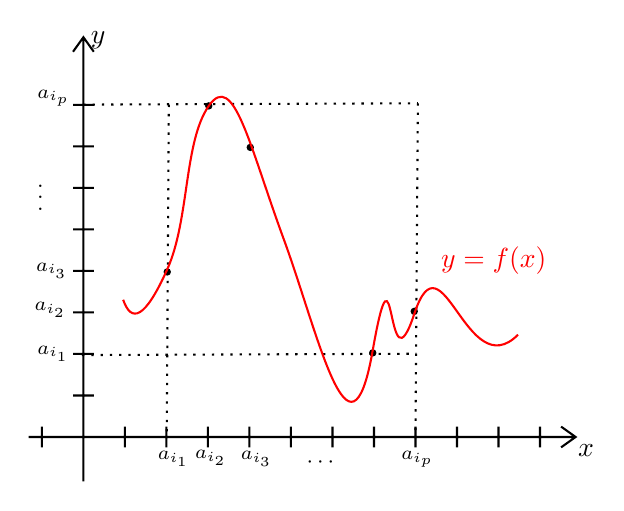
\begin{tikzpicture}[x=0.75pt,y=0.75pt,yscale=-1,xscale=1]
				%uncomment if require: \path (0,300); %set diagram left start at 0, and has height of 300
				
				%Shape: Axis 2D [id:dp6481518428974078] 
				\draw  (53.5,200.1) -- (317,200.1)(79.85,7.5) -- (79.85,221.5) (310,195.1) -- (317,200.1) -- (310,205.1) (74.85,14.5) -- (79.85,7.5) -- (84.85,14.5) (99.85,195.1) -- (99.85,205.1)(119.85,195.1) -- (119.85,205.1)(139.85,195.1) -- (139.85,205.1)(159.85,195.1) -- (159.85,205.1)(179.85,195.1) -- (179.85,205.1)(199.85,195.1) -- (199.85,205.1)(219.85,195.1) -- (219.85,205.1)(239.85,195.1) -- (239.85,205.1)(259.85,195.1) -- (259.85,205.1)(279.85,195.1) -- (279.85,205.1)(299.85,195.1) -- (299.85,205.1)(59.85,195.1) -- (59.85,205.1)(74.85,180.1) -- (84.85,180.1)(74.85,160.1) -- (84.85,160.1)(74.85,140.1) -- (84.85,140.1)(74.85,120.1) -- (84.85,120.1)(74.85,100.1) -- (84.85,100.1)(74.85,80.1) -- (84.85,80.1)(74.85,60.1) -- (84.85,60.1)(74.85,40.1) -- (84.85,40.1) ;
				\draw   ;
				%Straight Lines [id:da34830364825233673] 
				\draw  [dash pattern={on 0.84pt off 2.51pt}]  (121,40) -- (120,200) ;
				%Straight Lines [id:da21301944065434042] 
				\draw  [dash pattern={on 0.84pt off 2.51pt}]  (241,39.33) -- (239.83,200.03) ;
				%Straight Lines [id:da38423440107926] 
				\draw  [dash pattern={on 0.84pt off 2.51pt}]  (79.83,39.97) -- (241,39.33) ;
				%Straight Lines [id:da28398829303809614] 
				\draw  [dash pattern={on 0.84pt off 2.51pt}]  (79.17,160.63) -- (240.33,160) ;
				%Shape: Circle [id:dp7463394320389365] 
				\draw  [fill={rgb, 255:red, 0; green, 0; blue, 0 }  ,fill opacity=1 ] (119,120.58) .. controls (119,119.89) and (119.56,119.33) .. (120.25,119.33) .. controls (120.94,119.33) and (121.5,119.89) .. (121.5,120.58) .. controls (121.5,121.27) and (120.94,121.83) .. (120.25,121.83) .. controls (119.56,121.83) and (119,121.27) .. (119,120.58) -- cycle ;
				%Shape: Circle [id:dp6684633384567282] 
				\draw  [fill={rgb, 255:red, 0; green, 0; blue, 0 }  ,fill opacity=1 ] (139,40.58) .. controls (139,39.89) and (139.56,39.33) .. (140.25,39.33) .. controls (140.94,39.33) and (141.5,39.89) .. (141.5,40.58) .. controls (141.5,41.27) and (140.94,41.83) .. (140.25,41.83) .. controls (139.56,41.83) and (139,41.27) .. (139,40.58) -- cycle ;
				%Shape: Circle [id:dp10454278311396448] 
				\draw  [fill={rgb, 255:red, 0; green, 0; blue, 0 }  ,fill opacity=1 ] (159,60.58) .. controls (159,59.89) and (159.56,59.33) .. (160.25,59.33) .. controls (160.94,59.33) and (161.5,59.89) .. (161.5,60.58) .. controls (161.5,61.27) and (160.94,61.83) .. (160.25,61.83) .. controls (159.56,61.83) and (159,61.27) .. (159,60.58) -- cycle ;
				%Shape: Circle [id:dp2963444429880262] 
				\draw  [fill={rgb, 255:red, 0; green, 0; blue, 0 }  ,fill opacity=1 ] (218,159.58) .. controls (218,158.89) and (218.56,158.33) .. (219.25,158.33) .. controls (219.94,158.33) and (220.5,158.89) .. (220.5,159.58) .. controls (220.5,160.27) and (219.94,160.83) .. (219.25,160.83) .. controls (218.56,160.83) and (218,160.27) .. (218,159.58) -- cycle ;
				%Shape: Circle [id:dp8857686056743208] 
				\draw  [fill={rgb, 255:red, 0; green, 0; blue, 0 }  ,fill opacity=1 ] (238,139.58) .. controls (238,138.89) and (238.56,138.33) .. (239.25,138.33) .. controls (239.94,138.33) and (240.5,138.89) .. (240.5,139.58) .. controls (240.5,140.27) and (239.94,140.83) .. (239.25,140.83) .. controls (238.56,140.83) and (238,140.27) .. (238,139.58) -- cycle ;
				%Curve Lines [id:da692684928373148] 
				\draw [color={rgb, 255:red, 255; green, 0; blue, 0 }  ,draw opacity=1 ]   (99,134) .. controls (103,145.33) and (109.5,143.33) .. (120.25,119.33) .. controls (131,95.33) and (128.21,57.87) .. (140.25,40.58) .. controls (152.29,23.29) and (159.67,59.33) .. (176.33,104.67) .. controls (193,150) and (208.17,221.33) .. (219.25,158.33) .. controls (230.33,95.33) and (225.67,182) .. (239.25,140.83) .. controls (252.83,99.67) and (264.25,175.83) .. (289.25,150.83) ;
				
				% Text Node
				\draw (114.21,205.36) node [anchor=north west][inner sep=0.75pt]  [font=\scriptsize]  {$a_{i_{1}}$};
				% Text Node
				\draw (132.21,205.03) node [anchor=north west][inner sep=0.75pt]  [font=\scriptsize]  {$a_{i_{2}}$};
				% Text Node
				\draw (154.21,205.36) node [anchor=north west][inner sep=0.75pt]  [font=\scriptsize]  {$a_{i_{3}}$};
				% Text Node
				\draw (185.94,208.38) node [anchor=north west][inner sep=0.75pt]  [font=\footnotesize]  {$\cdots $};
				% Text Node
				\draw (231.55,205.36) node [anchor=north west][inner sep=0.75pt]  [font=\scriptsize]  {$a_{i_{p}}$};
				% Text Node
				\draw (56.21,154.7) node [anchor=north west][inner sep=0.75pt]  [font=\scriptsize]  {$a_{i_{1}}$};
				% Text Node
				\draw (54.88,133.7) node [anchor=north west][inner sep=0.75pt]  [font=\scriptsize]  {$a_{i_{2}}$};
				% Text Node
				\draw (55.55,114.7) node [anchor=north west][inner sep=0.75pt]  [font=\scriptsize]  {$a_{i_{3}}$};
				% Text Node
				\draw (56,69.4) node [anchor=north west][inner sep=0.75pt]  [font=\footnotesize]  {$\vdots $};
				% Text Node
				\draw (56.21,31.36) node [anchor=north west][inner sep=0.75pt]  [font=\scriptsize]  {$a_{i_{p}}$};
				% Text Node
				\draw (316.67,202.07) node [anchor=north west][inner sep=0.75pt]    {$x$};
				% Text Node
				\draw (82,3.4) node [anchor=north west][inner sep=0.75pt]    {$y$};
				% Text Node
				\draw (250.67,107.07) node [anchor=north west][inner sep=0.75pt]  [color={rgb, 255:red, 252; green, 0; blue, 0 }  ,opacity=1 ]  {$y=f( x)$};
				
				
			\end{tikzpicture}
		\caption{Ilustração gráfica.}
		\end{figure}
		
%\end{exercise}